\documentclass[11pt,a4paper]{article}

\usepackage[margin=2.5cm]{geometry}
\usepackage{booktabs}
\usepackage{float}
\usepackage{tabularx}
\usepackage{array}
\usepackage{enumitem}
\usepackage{totcount}
\usepackage{fancyhdr}
\usepackage{lastpage}
\usepackage{needspace}
\usepackage{tikz}
\usetikzlibrary{positioning}
\usepackage[hidelinks]{hyperref}
\setlength{\emergencystretch}{1.5em}

% Section numbers in the same style as the ConOps: 1.0, 1.1.
\renewcommand{\thesection}{\arabic{section}.0}
\renewcommand{\thesubsection}{\arabic{section}.\arabic{subsection}}

% Controlled-document header on every page.
\newcommand{\docref}{Reference TBD}
\newcommand{\docrev}{Issue 1, Rev.~0 --- DRAFT}
\pagestyle{fancy}
\fancyhf{}
\lhead{\small Remote Controller with Fail-Safe Update --- Hazard Analysis}
\rhead{\small \docrev}
\lfoot{\small \docref}
\rfoot{\small Page \thepage\ of \pageref{LastPage}}

% Open items. TBD = not known. TBR = proposal awaiting the author's
% acceptance. Listed in App. A; totals counted, not typed.
\newtotcounter{tbd}
\newtotcounter{tbr}
\newcommand{\tbditem}[2]{\refstepcounter{tbd}\label{tbd:#1}\item[TBD-\thetbd] #2}
\newcommand{\tbritem}[2]{\refstepcounter{tbr}\label{tbr:#1}\item[TBR-\thetbr] #2}
\newcommand{\tbd}[1]{\mbox{\textbf{[\hyperref[tbd:#1]{TBD-\ref*{tbd:#1}}]}}}
\newcommand{\tbr}[1]{\mbox{\textbf{[\hyperref[tbr:#1]{TBR-\ref*{tbr:#1}}]}}}

\setlist[description]{style=multiline,leftmargin=2cm,nosep,font=\normalfont\bfseries}
\setlist[itemize]{nosep}
\setlist[enumerate]{nosep}

% One hazard report: ID, hazard, severity, software role.
\newcommand{\hazard}[4]{\par\needspace{8\baselineskip}\medskip
  \noindent\textbf{#1\enspace #2}\par
  \noindent Severity: #3.\quad Software: #4.\par\smallskip}
\newenvironment{hazfields}{\begin{description}[leftmargin=3.3cm]}{\end{description}}
\newenvironment{hazlist}{\begin{enumerate}[label=(\alph*),leftmargin=*,topsep=0pt]}{\end{enumerate}}

% Fault tree symbols [4,~Table 4-1, p. 34]. Each gate pic has its output at
% the origin and its inputs below.
\tikzset{
  ev/.style={draw, rectangle, align=center, font=\scriptsize, inner sep=2pt,
    minimum height=1.05cm},
  basic/.style={draw, circle, minimum size=0.3cm, inner sep=0pt},
  andgate/.pic={\draw[thick] (-0.3,-0.7) -- (-0.3,-0.3) arc (180:0:0.3)
    -- (0.3,-0.7) -- cycle;},
  orgate/.pic={\draw[thick] (-0.3,-0.7) .. controls (-0.3,-0.3) and
    (-0.15,-0.1) .. (0,0) .. controls (0.15,-0.1) and (0.3,-0.3) ..
    (0.3,-0.7) .. controls (0.15,-0.58) and (-0.15,-0.58) .. (-0.3,-0.7)
    -- cycle;}
}

\begin{document}

\thispagestyle{fancy}
\begin{center}
{\LARGE\bfseries Remote Controller with Fail-Safe Update\par}
\vspace{0.4em}
{\Large Hazard Analysis\par}
\vspace{1em}
\begin{tabular}{@{}ll@{}}
Reference & TBD \tbd{ref} \\
Issue / revision & Issue 1, Revision 0 --- DRAFT \\
Date & 10 October 2026 \\
Author & Andrew Toma \\
Open items & \total{tbd} TBD, \total{tbr} TBR (App.~A) \\
\end{tabular}
\end{center}

\subsection*{Document change record}
\begin{tabular}{@{}llll@{}}
\toprule
Issue & Rev. & Date & Change \\
\midrule
1 & 0 & 2026-10-10 & First draft \\
\bottomrule
\end{tabular}

% ===========================================================================
\section{Purpose and Scope}
This document identifies the hazards of the System, the causes of each, its
severity, and the controls proposed against it. It is the Phase~0 and Phase~1
delivery of the hazard analysis, combined as for a small project: the top
hazards and causes, then all known hazards with their causes and controls
[2,~Sec.~4].

The controls are proposals; the requirements turn them into rules. The
verification of each control is added in the Phase~2 update, once a design
exists [2,~Sec.~3.1]. This document also decides which software is
safety-critical, which the Software Classification left open
[6,~Sec.~4.0].

The analysis covers the software items of the Software Classification in
operation [6,~Sec.~3.0]. Bench and build tools are covered where they can
affect operation.

% ===========================================================================
\section{Documents}
\noindent [1] NASA, \emph{Software Assurance and Software Safety Standard},
NASA-STD-8739.8B, 2022. Causes cite App.~A, Table~2, pp.~62--68.

\noindent [2] NASA, \emph{NASA Software Engineering Handbook}, NASA-HDBK-2203,
Version~D, Topic 8.58 ``Software Safety and Hazard Analysis''.

\noindent [3] NASA, \emph{NASA Software Engineering Handbook}, NASA-HDBK-2203,
Version~D, Topic 8.05 ``SW Failure Modes and Effects Analysis''.

\noindent [4] NASA, \emph{Fault Tree Handbook with Aerospace Applications},
Version~1.1, August 2002.

\noindent [5] \emph{Remote Controller with Fail-Safe Update --- Concept of
Operations}, Issue~1, Revision~0, Draft.

\noindent [6] \emph{Remote Controller with Fail-Safe Update --- Software
Classification}, Issue~1, Revision~0, Draft.

% ===========================================================================
\section{Ground Rules}
\begin{itemize}
\item \textbf{Hazard:} a state, or a set of conditions, with the potential to
  cause harm [1,~p.~13].
\item \textbf{Sources:} the ConOps and the list of software causes of hazards
  [1,~App.~A, Table~2, pp.~62--68]. Numbers of objectives (O), assumptions (A),
  constraints (C), risks (R), capabilities and scenarios refer to the ConOps
  [5,~Secs.~1.1.2, 3.1, 3.5, 6.0 and 8.0].
\item \textbf{Points of view:} functional, operational, software,
  environment, human and organizational [2,~Sec.~3.2.2]. The physical view
  needs the architecture and is added with it.
\item \textbf{Severity:} the worst credible effect, rated as if no control
  worked \tbr{severity}.
\item \textbf{Credible failures:} up to two at once for a catastrophic hazard,
  and one for a critical hazard [3,~Sec.~3.1] \tbr{credible}.
\item \textbf{Likelihood:} not rated yet; it depends on the design
  \tbd{likelihood}.
\item \textbf{Controls:} a control with a scenario number comes from the
  ConOps. A control without one is new and proposed here.
\end{itemize}

\medskip
\noindent\textbf{Legend: severity} (names from [3,~Sec.~6])
\begin{description}[leftmargin=4cm]
\item[CATASTROPHIC] The controller is lost, or can no longer be commanded,
  observed or corrected, for the rest of the mission.
\item[CRITICAL] The controller acts against the operator's intent, or cannot
  be commanded, observed or corrected until the ground acts.
\item[MARGINAL] A function is degraded or interrupted, but none of the above
  happens.
\item[NEGLIGIBLE] No function is degraded; the operator has extra work or a
  delay.
\end{description}

\medskip
\noindent\textbf{Legend: software role} [2,~Sec.~3.2.2]
\begin{description}[leftmargin=4cm]
\item[CAUSE] A software fault can lead to the hazard.
\item[CONTROL] Software prevents the hazard.
\item[MITIGATION] Software limits the effect once the hazard occurs.
\item[MONITOR] Software detects and reports the hazard.
\end{description}

% ===========================================================================
\section{Hazard List}
The hazards in order of severity \tbr{hazards}:

\begin{table}[H]
\centering
\begin{tabularx}{\textwidth}{@{}l>{\raggedright\arraybackslash}Xl@{}}
\toprule
ID & Hazard & Severity \\
\midrule
H-1  & The controller is left with no firmware it can run, and cannot be restored & CATASTROPHIC \\
H-2  & Firmware not released by the operator runs on the controller & CATASTROPHIC \\
H-3  & New firmware can no longer reach the controller & CATASTROPHIC \\
H-4  & The controller can no longer be commanded or observed & CATASTROPHIC \\
H-5  & Someone other than the operator commands the System & CATASTROPHIC \\
H-6  & A command is acted on in a form or at a time the operator did not intend & CRITICAL \\
H-7  & Defective firmware released by the operator is confirmed & CRITICAL \\
H-8  & The controller stops working between contacts and is not brought back & CRITICAL \\
H-9  & The ground is shown a false state of the System & CRITICAL \\
H-10 & A fault between contacts never reaches the ground & CRITICAL \\
H-11 & A valid command is not acted on, and the ground is not told & CRITICAL \\
H-12 & A test function acts outside a test & CRITICAL \\
H-13 & A fault response is taken when there is no fault & MARGINAL \\
H-14 & An update cannot be completed & MARGINAL \\
H-15 & Health reports are lost & MARGINAL \\
H-16 & Reports reach the ground later than planned & NEGLIGIBLE \\
H-17 & A command is refused with a wrong or unclear reason & NEGLIGIBLE \\
\bottomrule
\end{tabularx}
\end{table}

% ===========================================================================
\section{Top-Down Analysis}
Figure~\ref{fig:tree} develops the worst hazard, H-1, from the top down.

\begin{figure}[H]
\centering
\resizebox{\textwidth}{!}{%
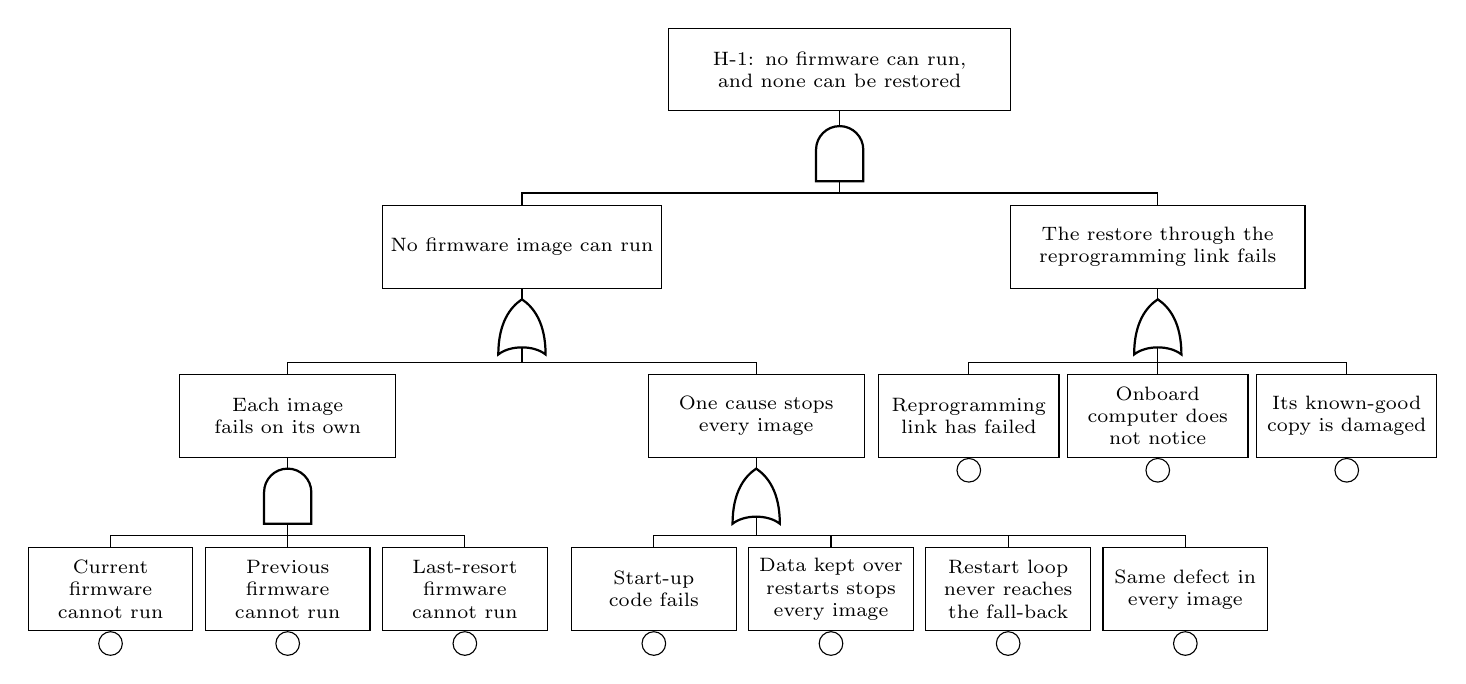
\begin{tikzpicture}
% Levels: event tops at 0.5, -1.75, -3.9, -6.1; gate outputs at -0.75,
% -2.95, -5.1. Lines leave a gate's base and meet a bus above the events.
\node[ev, anchor=north, text width=4.2cm] (T) at (1.66,0.5) {H-1: no firmware can run, and none can be restored};
\pic at (1.66,-0.75) {andgate};
\draw (T.south) -- (1.66,-0.75);
\node[ev, anchor=north, text width=3.4cm] (E1) at (-2.375,-1.75) {No firmware image can run};
\node[ev, anchor=north, text width=3.6cm] (E2) at (5.7,-1.75) {The restore through the reprogramming link fails};
\draw (1.66,-1.45) -- (1.66,-1.6) -| (E1.north);
\draw (1.66,-1.6) -| (E2.north);
\pic at (-2.375,-2.95) {orgate};
\pic at (5.7,-2.95) {orgate};
\draw (E1.south) -- (-2.375,-2.95);
\draw (E2.south) -- (5.7,-2.95);
% Two ways no image can run.
\node[ev, anchor=north, text width=2.6cm] (E3) at (-5.35,-3.9) {Each image fails on its own};
\node[ev, anchor=north, text width=2.6cm] (E4) at (0.6,-3.9) {One cause stops every image};
\draw (-2.375,-3.55) -- (-2.375,-3.75) -| (E3.north);
\draw (-2.375,-3.75) -| (E4.north);
% Why the restore fails.
\foreach \x/\t [count=\i] in {3.3/Reprogramming link has failed,
    5.7/Onboard computer does not notice,
    8.1/Its known-good copy is damaged} {
  \node[ev, anchor=north, text width=2.15cm] (R\i) at (\x,-3.9) {\t};
  \node[basic, below=0pt of R\i] {};
  \draw (5.7,-3.55) -- (5.7,-3.75) -| (R\i.north);
}
\pic at (-5.35,-5.1) {andgate};
\pic at (0.6,-5.1) {orgate};
\draw (E3.south) -- (-5.35,-5.1);
\draw (E4.south) -- (0.6,-5.1);
% Basic events.
\foreach \x/\t [count=\i] in {-7.6/Current firmware cannot run,
    -5.35/Previous firmware cannot run,
    -3.1/Last-resort firmware cannot run} {
  \node[ev, anchor=north, text width=1.95cm] (A\i) at (\x,-6.1) {\t};
  \node[basic, below=0pt of A\i] {};
  \draw (-5.35,-5.8) -- (-5.35,-5.95) -| (A\i.north);
}
\foreach \x/\t [count=\i] in {-0.7/Start-up code fails,
    1.55/Data kept over restarts stops every image,
    3.8/Restart loop never reaches the fall-back,
    6.05/Same defect in every image} {
  \node[ev, anchor=north, text width=1.95cm] (B\i) at (\x,-6.1) {\t};
  \node[basic, below=0pt of B\i] {};
  \draw (0.6,-5.7) -- (0.6,-5.95) -| (B\i.north);
}
\end{tikzpicture}}
\caption{Fault tree of H-1. Symbols as in [4,~Table 4-1, p.~34].}
\label{fig:tree}
\end{figure}

\noindent\textbf{Legend: symbols}
\begin{description}[leftmargin=3.4cm]
\item[Rectangle] An event developed further by the gate below it.
\item[Circle] A basic event, not developed further here.
\item[AND gate] Flat base: the event above occurs if all events below occur.
\item[OR gate] Curved base: the event above occurs if at least one event below
  occurs.
\end{description}

\medskip
A minimal cut set is the smallest combination of basic events that causes the
top event [4,~Sec.~1.3, p.~3]. H-1 has two kinds:
\begin{itemize}
\item \textbf{Four events:} the current, previous and last-resort firmware all
  fail on their own, and the restore fails.
\item \textbf{Two events:} one cause stops every image, and the restore
  fails.
\end{itemize}
Two failures at once are credible for a catastrophic hazard (Section~3.0). The
causes that stop every image are therefore the weakest point of H-1: they
defeat three layers of firmware with one event.

% ===========================================================================
\section{Bottom-Up Analysis}
Before a design exists, the components examined are the System's functions
[3,~Sec.~4]. Each function is examined for each way it can fail, and each
failure is traced to the hazard it leads to.

\begin{table}[H]
\centering
\small
\begin{tabularx}{\textwidth}{@{}>{\raggedright\arraybackslash}Xllll@{}}
\toprule
Function & OMITTED & INCORRECT & UNWANTED & MISTIMED \\
\midrule
\multicolumn{5}{@{}l}{\itshape Telemetry (Capability-1)} \\
Make health and event reports & H-10, H-15 & H-9 & H-4, H-15 & H-9 \\
Time-tag and store reports & H-10, H-15 & H-9 & H-15 & H-9 \\
Send reports down & H-10, H-15 & H-9 & H-16 & H-16 \\
Keep received reports on the ground & H-10, H-15 & H-9 & NONE & NONE \\
\multicolumn{5}{@{}l}{\itshape Command handling (Capability-2)} \\
Prepare and check commands on the ground & H-6 & H-6 & H-6 & H-6 \\
Check commands onboard & H-5, H-6 & H-6, H-11, H-17 & NONE & H-4, H-6, H-11 \\
Hold armed and scheduled commands & H-11 & H-6 & H-6 & H-6 \\
Run commands & H-11 & H-6 & H-5, H-6 & H-6 \\
Answer and log commands & H-11 & H-9, H-17 & H-9 & H-16 \\
\multicolumn{5}{@{}l}{\itshape Fault handling (Capability-3)} \\
Detect faults & H-8, H-10 & H-10, H-13 & H-13 & H-8 \\
Respond to faults & H-8 & H-1, H-4, H-13 & H-13 & H-8 \\
\multicolumn{5}{@{}l}{\itshape Update (Capability-4)} \\
Prepare and check firmware releases & H-7 & H-3, H-7 & H-2 & NONE \\
Receive and check firmware & H-1, H-2 & H-2, H-3, H-14 & H-14 & H-2 \\
Install firmware and switch & H-14 & H-1 & H-6 & H-1 \\
Judge and confirm new firmware & H-13 & H-3, H-7 & H-7 & H-7, H-13 \\
Fall back to working firmware & H-1, H-8 & H-1, H-2 & H-13 & H-8, H-13 \\
Restore through the reprogramming link & H-1 & H-1, H-2 & H-13 & H-1 \\
\multicolumn{5}{@{}l}{\itshape Test (Capability-5)} \\
Inject faults & NONE & NONE & H-12 & H-12 \\
\bottomrule
\end{tabularx}
\end{table}

\noindent\textbf{Legend: failure mode}
\begin{description}[leftmargin=3.4cm]
\item[OMITTED] The function is not performed.
\item[INCORRECT] The function is performed with a wrong result.
\item[UNWANTED] The function is performed when it must not be.
\item[MISTIMED] The function is performed too early, too late or out of order.
\item[NONE] The failure leads to no hazard.
\end{description}

\medskip
Every failure leads to a hazard of the list in Section~4.0, or to none.

% ===========================================================================
\section{Common Causes}
A common cause defeats several controls at once; it can negate a redundancy
[4,~Sec.~1.3, p.~3]. It includes the same defect in software that runs in
more than one place [1,~App.~A.1.1, p.~62]. The common causes found are:

\noindent\textbf{Wrong onboard clock.} Expiry, arm time-outs, scheduled commands,
time-tags and the trial time limit all depend on the onboard clock
[1,~p.~65]. Hazards: H-4, H-6, H-9, H-11, H-13.\par\smallskip
\noindent\textbf{Code shared by every image.} The start-up code, and any defect common to
the current, previous and last-resort firmware, stops all of them at once.
Hazards: H-1, H-8.\par\smallskip
\noindent\textbf{Data kept over restarts.} Stored settings, counters and flags survive a
restart. A wrong value can stop every image or keep a wrong state
[1,~p.~64]. Hazards: H-1, H-6, H-13.\par\smallskip
\noindent\textbf{One power supply.} The onboard computer and the controller share the
spacecraft power supply [5,~Sec.~3.3]. A power loss stops the controller and
the computer that would restore it, and interrupts reports and commands.
Hazards: H-1, H-8, H-10, H-11, H-15.\par\smallskip
\noindent\textbf{Same software at both data-link ends.} One defect can cut both
connections (R-1) [1,~p.~66]. Hazards: H-4.\par\smallskip
\noindent\textbf{One means of proving origin.} If one means proves that both commands and
firmware come from the operator, its disclosure opens both. Hazards: H-2,
H-5.\par\smallskip
\noindent\textbf{Radiation.} Bit errors can strike stored firmware, running memory, stored
reports, held commands and the arm state (A-5) [1,~p.~63]. Hazards: H-1, H-6,
H-8, H-9, H-10.\par\smallskip
\noindent\textbf{One set of build tools.} The same tools build every image; a tool defect
enters all of them. Hazards: H-1, H-7, H-12.\par\smallskip
\noindent\textbf{Onboard computer software that cannot be updated.} It stays fixed for the
mission [5,~Sec.~5.0], so a defect in it is never corrected. Hazards: H-1,
H-3, H-4.\par\smallskip
\noindent\textbf{One engineer and AI-drafted code.} The same misunderstanding can enter a
function and the check meant to catch it (C-3, R-2) [1,~p.~67]. Hazards:
all.\par\smallskip

% ===========================================================================
\section{Hazard Reports}
Each report gives the conditions, causes, worst effect, proposed controls, how
the controls can fail, and the common causes that defeat them [2,~Sec.~4].

% ---------------------------------------------------------------- H-1
\hazard{H-1}{The controller is left with no firmware it can run, and cannot be restored.}{CATASTROPHIC}{CAUSE, CONTROL}
\begin{hazfields}
\item[When] During an update, at any restart, or when a restore is needed.
\item[Causes] \begin{hazlist}
  \item Power is lost while firmware is written (Scenario-600) [1,~p.~63].
  \item A bit error changes stored firmware (Scenario-610) [1,~p.~63].
  \item An update writes over the firmware the controller would fall back to
    [1,~p.~65].
  \item The new and the previous firmware both fail (Scenario-460).
  \item The last-resort firmware has changed unnoticed by the time it is
    needed [1,~p.~63].
  \item A restart loop never reaches the fall-back [1,~p.~64].
  \item The start-up code fails, or its stored copy is damaged [1,~p.~63].
  \item The reprogramming link has failed, or the onboard computer does not
    notice that a restore is needed (Scenario-520).
  \item The onboard computer's known-good copy of the firmware is damaged
    [1,~p.~63].
  \end{hazlist}
\item[Effect] The controller is lost for the rest of the mission; nobody can
  reach it (A-1).
\item[Controls] \begin{enumerate}[leftmargin=*,topsep=0pt]
  \item An update never writes over the firmware the controller would fall back
    to (Scenario-600).
  \item Every firmware image is checked before it runs (Scenario-610).
  \item Failed starts are counted; after a set number, the controller returns
    to its previous firmware (Scenario-440).
  \item A last-resort firmware that updates never replace (Scenario-460).
  \item A restore through the reprogramming link, which does not depend on the
    controller's software (Scenario-480).
  \item Stored firmware and the reprogramming link are checked between uses,
    so a hidden fault is reported before it is needed.
  \end{enumerate}
\item[Control fails if] The image check passes damaged firmware; the
  failed-start count is lost at each restart; the last-resort firmware shares
  the defect that stops the others.
\item[Common causes] Code shared by every image; data kept over restarts; one
  power supply; radiation; one set of build tools; onboard computer software
  that cannot be updated.
\end{hazfields}

% ---------------------------------------------------------------- H-2
\hazard{H-2}{Firmware not released by the operator runs on the controller.}{CATASTROPHIC}{CONTROL}
\begin{hazfields}
\item[When] During an update, a fall-back or a restore.
\item[Causes] \begin{hazlist}
  \item Firmware not from the operator arrives (Scenario-410) [1,~p.~67].
  \item Firmware is changed after it is checked, in transfer or in storage
    [1,~p.~63].
  \item Firmware older than the minimum version, which the operator no longer
    releases, is sent again (Scenario-420).
  \item The means of proving that firmware comes from the operator is
    disclosed.
  \item A fall-back or a restore starts an image that was never released.
  \end{hazlist}
\item[Effect] Firmware of unknown behaviour runs the controller. It can refuse
  further updates and report a false state. The restore is used only when no
  firmware can run (Scenario-480), so firmware that runs is never removed.
\item[Controls] \begin{enumerate}[leftmargin=*,topsep=0pt]
  \item The onboard computer refuses firmware that is not released by the
    operator (Scenario-410), damaged (Scenario-400), older than the minimum
    version (Scenario-420), or built for another controller (Scenario-360).
  \item The controller checks firmware again before it runs it
    (Scenario-610).
  \item The operator can order a restore through the reprogramming link while
    firmware is running.
  \end{enumerate}
\item[Control fails if] The check accepts what it should refuse; the check is
  made before the last transfer, not after it.
\item[Common causes] One means of proving origin; radiation.
\end{hazfields}

% ---------------------------------------------------------------- H-3
\hazard{H-3}{New firmware can no longer reach the controller.}{CATASTROPHIC}{CAUSE, CONTROL}
\begin{hazfields}
\item[When] After an update is confirmed, or after a fault in the onboard
  computer.
\item[Causes] \begin{hazlist}
  \item Confirmed firmware runs, but cannot receive new firmware.
  \item A defect in the onboard computer's update path.
  \item A stored minimum version or controller identity is wrong, so all new
    firmware is refused [1,~p.~67].
  \item Storage for firmware on the onboard computer stays full [1,~p.~66].
  \end{hazlist}
\item[Effect] The controller can no longer be corrected for the rest of the
  mission.
\item[Controls] \begin{enumerate}[leftmargin=*,topsep=0pt]
  \item New firmware runs a trial before it is confirmed (Scenario-430 to
    Scenario-450).
  \item New firmware is judged good only after it has received firmware itself.
  \item The last-resort firmware can always receive new firmware.
  \item The operator can order a return to the last-resort firmware.
  \end{enumerate}
\item[Control fails if] The trial does not test the update path; the defect is
  in the onboard computer, which no control can reach.
\item[Common causes] Onboard computer software that cannot be updated; data
  kept over restarts.
\end{hazfields}

% ---------------------------------------------------------------- H-4
\hazard{H-4}{The controller can no longer be commanded or observed.}{CATASTROPHIC}{CAUSE, CONTROL}
\begin{hazfields}
\item[When] At any time.
\item[Causes] \begin{hazlist}
  \item Both data-link connections fail (Scenario-510).
  \item One software defect cuts both connections (R-1) [1,~p.~66].
  \item A controller that never stops sending blocks the data link
    [1,~p.~63].
  \item The onboard clock is wrong, so every command is refused as expired,
    including the one that would correct the clock [1,~p.~65].
  \item The ground loses the means of proving that commands come from the
    operator, so no command is accepted.
  \item A fault response marks both connections failed (H-13).
  \end{hazlist}
\item[Effect] The controller runs on with its current firmware, but nobody can
  command or observe it for the rest of the mission.
\item[Controls] \begin{enumerate}[leftmargin=*,topsep=0pt]
  \item Two separate data-link connections; one is enough (O-3,
    Scenario-500).
  \item The loss of a connection is reported (Scenario-500, Scenario-510).
  \item The reprogramming link stays usable (Scenario-510).
  \item The command that corrects the onboard clock does not depend on the
    onboard clock.
  \end{enumerate}
\item[Control fails if] Both connections fail from one cause. No control yet
  covers a lost means of proving origin.
\item[Common causes] Same software at both data-link ends; wrong onboard clock;
  onboard computer software that cannot be updated.
\end{hazfields}

% ---------------------------------------------------------------- H-5
\hazard{H-5}{Someone other than the operator commands the System.}{CATASTROPHIC}{CONTROL}
\begin{hazfields}
\item[When] During a contact, or at any time for a source on the spacecraft.
\item[Causes] \begin{hazlist}
  \item A command not from the operator arrives (Scenario-300) [1,~p.~67].
  \item The means of proving that a command comes from the operator is
    disclosed.
  \item Someone other than the operator uses the operator interface; no second
    person checks a command (A-4).
  \item A command arrives from an unexpected system on the spacecraft
    [1,~p.~62].
  \end{hazlist}
\item[Effect] Another party can do anything the operator can, and hide it.
  Control of the controller is lost for the rest of the mission.
\item[Controls] \begin{enumerate}[leftmargin=*,topsep=0pt]
  \item Every command is proven to come from the operator; any other is refused
    and logged (O-2, Scenario-300).
  \item Only the operator can use the operator interface.
  \end{enumerate}
\item[Control fails if] The means of proof is disclosed; the check accepts what
  it should refuse.
\item[Common causes] One means of proving origin.
\end{hazfields}

% ---------------------------------------------------------------- H-6
\hazard{H-6}{A command is acted on in a form or at a time the operator did not intend.}{CRITICAL}{CAUSE, CONTROL}
\begin{hazfields}
\item[When] While a command is checked, held or run.
\item[Causes] \begin{hazlist}
  \item A command is changed in transfer [1,~p.~62].
  \item An old command is sent again (Scenario-300).
  \item A command is run twice after a lost answer (Scenario-350).
  \item A command not allowed in the current mode arrives (Scenario-310)
    [1,~p.~63].
  \item A command with impossible values arrives (Scenario-320) [1,~p.~62].
  \item A dangerous command arrives without a valid arm (Scenario-330,
    Scenario-335) [1,~p.~63].
  \item A command arrives after its expiry (Scenario-340) [1,~p.~63].
  \item A scheduled command runs at the wrong time, or again after a restart
    [1,~p.~64].
  \item A bit error changes a held command or the arm state [1,~p.~63].
  \item The ground software builds a wrong command, or the operator enters one
    (A-4) [1,~p.~63].
  \end{hazlist}
\item[Effect] The controller does what the operator did not intend, and the
  ground learns of it only at the next contact.
\item[Controls] \begin{enumerate}[leftmargin=*,topsep=0pt]
  \item The onboard computer checks that every command is new, allowed in the
    current mode, has possible values and has not expired (Scenario-120).
  \item A dangerous command needs an arm, which expires (Scenario-330,
    Scenario-335).
  \item A command sent again is not run twice; the answer is ``already done''
    (Scenario-350).
  \item The ground software checks every command before it is sent
    (Scenario-120).
  \item Every command and its answers are logged (Scenario-120).
  \end{enumerate}
\item[Control fails if] The checks use a wrong onboard clock; a held command or
  the arm state changes after it is checked.
\item[Common causes] Wrong onboard clock; radiation; data kept over restarts.
\end{hazfields}

% ---------------------------------------------------------------- H-7
\hazard{H-7}{Defective firmware released by the operator is confirmed.}{CRITICAL}{CAUSE, CONTROL}
\begin{hazfields}
\item[When] During the trial of new firmware, and after it is confirmed.
\item[Causes] \begin{hazlist}
  \item The trial does not exercise the defect.
  \item The wrong build is released [1,~p.~67].
  \item The release carries wrong configuration values [1,~p.~67].
  \item Firmware built for a different controller is released (Scenario-360).
  \item The build tools put a defect into the firmware.
  \item Code is released without being fully tested [1,~p.~67].
  \end{hazlist}
\item[Effect] The controller misbehaves until a further update. If the defect
  stops updates, H-3 follows.
\item[Controls] \begin{enumerate}[leftmargin=*,topsep=0pt]
  \item New firmware not judged good within the trial time is given up
    (Scenario-430 to Scenario-450).
  \item Firmware built for another controller is refused (Scenario-360).
  \item The ground software checks every release before it is sent
    (Scenario-100).
  \item The operator can order a return to the previous firmware.
  \end{enumerate}
\item[Control fails if] The judgement checks too little; the trial is shorter
  than the time the defect takes to show.
\item[Common causes] One set of build tools; one engineer and AI-drafted code.
\end{hazfields}

% ---------------------------------------------------------------- H-8
\hazard{H-8}{The controller stops working between contacts and is not brought back.}{CRITICAL}{CAUSE, CONTROL, MONITOR}
\begin{hazfields}
\item[When] In any controller mode.
\item[Causes] \begin{hazlist}
  \item A bit error in the memory the controller runs from (Scenario-620)
    [1,~p.~63].
  \item The firmware hangs, deadlocks or overloads [1,~p.~63].
  \item The controller restarts but does not resume [1,~p.~63].
  \item The restart takes longer than the time to the next failure
    [1,~p.~64].
  \item The controller misbehaves when no command arrives for a long time
    [1,~p.~65].
  \item The onboard computer does not notice the silence, or its watching
    program has crashed (Scenario-520, Scenario-530).
  \end{hazlist}
\item[Effect] The controller's work stops until the ground acts at the next
  contact.
\item[Controls] \begin{enumerate}[leftmargin=*,topsep=0pt]
  \item The controller restarts on its own and resumes (Scenario-620).
  \item The onboard computer notices the silence, tries to bring the controller
    back, and records what it did (Scenario-520).
  \item A program on the onboard computer that crashes restarts and resumes
    (Scenario-530).
  \item New firmware that hangs is given up (Scenario-430).
  \end{enumerate}
\item[Control fails if] The controller's own restart and the onboard
  computer's watch fail from one fault.
\item[Common causes] Radiation; data kept over restarts; one power supply;
  code shared by every image.
\end{hazfields}

% ---------------------------------------------------------------- H-9
\hazard{H-9}{The ground is shown a false state of the System.}{CRITICAL}{CAUSE, CONTROL}
\begin{hazfields}
\item[When] At every contact.
\item[Causes] \begin{hazlist}
  \item Reports carry a wrong time-tag [1,~p.~64].
  \item Old reports are shown as current [1,~p.~63].
  \item A report is changed in storage or in transfer [1,~p.~62].
  \item An answer says ``done'' or ``already done'' for a command that did not
    run.
  \item The ground software stores or shows a report wrongly [1,~p.~62].
  \end{hazlist}
\item[Effect] The operator decides on false information: a harmful command can
  follow (H-6), or a fault is missed (H-10).
\item[Controls] \begin{enumerate}[leftmargin=*,topsep=0pt]
  \item The onboard computer time-tags every report (Scenario-110).
  \item Every report is checked for damage when it arrives.
  \item The ground software keeps every report received [5,~Sec.~3.2].
  \end{enumerate}
\item[Control fails if] The onboard clock is wrong; a report is damaged before
  its check is made.
\item[Common causes] Wrong onboard clock; radiation.
\end{hazfields}

% ---------------------------------------------------------------- H-10
\hazard{H-10}{A fault between contacts never reaches the ground.}{CRITICAL}{CAUSE, MONITOR}
\begin{hazfields}
\item[When] Between contacts.
\item[Causes] \begin{hazlist}
  \item The fault is not detected [1,~p.~66].
  \item It is detected, but no event report is made [1,~p.~65].
  \item The event report is lost: storage is full, a program crashes, or power
    is lost before it is stored (Scenario-210, Scenario-530).
  \item The ground loses it after it arrives.
  \end{hazlist}
\item[Effect] The ground does not know of the fault. Hidden faults pile up, for
  example a damaged last-resort firmware (H-1).
\item[Controls] \begin{enumerate}[leftmargin=*,topsep=0pt]
  \item Event reports are kept when storage is full (Scenario-210).
  \item No report is lost without the ground being told (O-5).
  \item Stored reports survive a power loss and a restart.
  \end{enumerate}
\item[Control fails if] Fault detection depends on the part that has failed.
\item[Common causes] One power supply; radiation.
\end{hazfields}

% ---------------------------------------------------------------- H-11
\hazard{H-11}{A valid command is not acted on, and the ground is not told.}{CRITICAL}{CAUSE, CONTROL}
\begin{hazfields}
\item[When] While a command is checked, held or run.
\item[Causes] \begin{hazlist}
  \item The command is lost in a full buffer [1,~p.~63].
  \item It is refused as expired because the onboard clock is wrong
    (Scenario-340).
  \item A scheduled command is lost at a restart (Scenario-130).
  \item Heavy traffic on the data link stops it getting through [1,~p.~63].
  \item Its answer is lost (Scenario-350).
  \end{hazlist}
\item[Effect] The operator believes an action was taken that was not; for
  example, a cancelled update goes on (Scenario-470).
\item[Controls] \begin{enumerate}[leftmargin=*,topsep=0pt]
  \item Every command gets two answers: received, then done with the result
    (Scenario-120).
  \item A refused command is answered with the reason (Scenario-310 to
    Scenario-340).
  \item Scheduled commands survive a restart.
  \end{enumerate}
\item[Control fails if] The answers are lost along with the command.
\item[Common causes] Wrong onboard clock; one power supply.
\end{hazfields}

% ---------------------------------------------------------------- H-12
\hazard{H-12}{A test function acts outside a test.}{CRITICAL}{CAUSE}
\begin{hazfields}
\item[When] In operation.
\item[Causes] \begin{hazlist}
  \item Fault-injection functions stay in the operating software
    [1,~p.~64].
  \item A wrong command, or one not from the operator, starts them.
  \end{hazlist}
\item[Effect] Power is cut, a data-link connection is broken, or the radio link
  is degraded during operation. Each is a cause of H-1 or H-4.
\item[Controls] \begin{enumerate}[leftmargin=*,topsep=0pt]
  \item Test functions are for verification only (Capability-5).
  \item Test functions are not part of the operating software.
  \end{enumerate}
\item[Control fails if] A bench build is released for operation [1,~p.~67].
\item[Common causes] One set of build tools.
\end{hazfields}

% ---------------------------------------------------------------- H-13
\hazard{H-13}{A fault response is taken when there is no fault.}{MARGINAL}{CAUSE}
\begin{hazfields}
\item[When] In any controller mode.
\item[Causes] \begin{hazlist}
  \item Fault detection reports a fault that is not there [1,~p.~66].
  \item The trial time is too short for good firmware to be judged good
    (Scenario-450).
  \item A failed-start count or a flag is not cleared [1,~p.~66].
  \end{hazlist}
\item[Effect] Good firmware is given up, the controller restarts for no
  reason, or a good data-link connection is marked failed. Repeated, it becomes
  a restart loop (H-1) or the loss of both connections (H-4).
\item[Controls] \begin{enumerate}[leftmargin=*,topsep=0pt]
  \item Every fault response is recorded and reported (Capability-3).
  \item A given-up update can be repeated (Scenario-600).
  \end{enumerate}
\item[Control fails if] The record of the response is lost with it.
\item[Common causes] Data kept over restarts; wrong onboard clock.
\end{hazfields}

% ---------------------------------------------------------------- H-14
\hazard{H-14}{An update cannot be completed.}{MARGINAL}{CAUSE, CONTROL}
\begin{hazfields}
\item[When] During an update.
\item[Causes] \begin{hazlist}
  \item The radio link is lost again and again during the upload
    (Scenario-200).
  \item A resumed upload is put together wrongly and refused.
  \item Storage on the onboard computer is full of reports (Scenario-210)
    [1,~p.~66].
  \item Good firmware is refused because the check is wrong.
  \end{hazlist}
\item[Effect] The current firmware keeps running; the correction waits. If it
  never completes, H-3 follows.
\item[Controls] \begin{enumerate}[leftmargin=*,topsep=0pt]
  \item An upload resumes from where it stopped (Scenario-200).
  \item A crashed program on the onboard computer resumes the update
    (Scenario-530).
  \item The operator can cancel an update (Scenario-470).
  \end{enumerate}
\item[Control fails if] The point where the upload stopped is stored wrongly.
\item[Common causes] Data kept over restarts.
\end{hazfields}

% ---------------------------------------------------------------- H-15
\hazard{H-15}{Health reports are lost.}{MARGINAL}{CAUSE, MITIGATION}
\begin{hazfields}
\item[When] Between contacts.
\item[Causes] \begin{hazlist}
  \item Storage fills during a long gap between contacts (Scenario-210).
  \item Power is lost, or a program crashes, before a report is stored.
  \item A bit error damages stored reports [1,~p.~62].
  \end{hazlist}
\item[Effect] The health history between contacts has gaps; a slow change can
  be missed. Event reports are covered by H-10.
\item[Controls] \begin{enumerate}[leftmargin=*,topsep=0pt]
  \item The oldest health reports are dropped first, and the ground is told how
    many and over what time span (Scenario-210).
  \end{enumerate}
\item[Control fails if] The count of dropped reports is itself lost.
\item[Common causes] One power supply; radiation.
\end{hazfields}

% ---------------------------------------------------------------- H-16
\hazard{H-16}{Reports reach the ground later than planned.}{NEGLIGIBLE}{CAUSE}
\begin{hazfields}
\item[When] At a contact after a long gap.
\item[Causes] \begin{hazlist}
  \item A contact is too short to send everything stored (A-3).
  \end{hazlist}
\item[Effect] No report is lost; the operator sees some of them a contact
  later.
\item[Controls] \begin{enumerate}[leftmargin=*,topsep=0pt]
  \item Event reports are sent before health reports.
  \end{enumerate}
\item[Control fails if] Event reports alone fill the contact.
\item[Common causes] None.
\end{hazfields}

% ---------------------------------------------------------------- H-17
\hazard{H-17}{A command is refused with a wrong or unclear reason.}{NEGLIGIBLE}{CAUSE}
\begin{hazfields}
\item[When] When a command is refused.
\item[Causes] \begin{hazlist}
  \item The ground and the onboard software use different lists of commands or
    reasons [1,~p.~66].
  \item Errors are handled differently in different places [1,~p.~63].
  \end{hazlist}
\item[Effect] The operator spends a contact finding out why, then sends the
  command again.
\item[Controls] \begin{enumerate}[leftmargin=*,topsep=0pt]
  \item One list of commands and refusal reasons, shared by the ground and the
    onboard software.
  \end{enumerate}
\item[Control fails if] The two copies of the list drift apart.
\item[Common causes] None.
\end{hazfields}

% ===========================================================================
\section{Must-Work and Must-Not-Work Functions}
The hazard reports identify the functions that must work and those that must
not work [1,~App.~A.1.2, p.~62].

\medskip
\noindent\textbf{Must work}
\begin{itemize}
\item Return to working firmware when new firmware fails (H-1).
\item Restore the controller through the reprogramming link (H-1, H-2).
\item Check every firmware image before it runs (H-1, H-2).
\item Refuse commands and firmware not from the operator (H-2, H-5).
\item Accept the command that corrects the onboard clock (H-4).
\item Detect and report faults between contacts (H-8, H-10).
\item Keep and send down every event report (H-10).
\item Answer every command (H-11).
\end{itemize}

\medskip
\noindent\textbf{Must not work}
\begin{itemize}
\item Write over the firmware the controller would fall back to, or over the
  last-resort firmware (H-1).
\item Run firmware not released by the operator (H-2).
\item Run a command not from the operator (H-5).
\item Run a dangerous command without a valid arm (H-6).
\item Run a command twice (H-6).
\item Confirm firmware that has not been judged good (H-7).
\item Inject faults outside a test (H-12).
\end{itemize}

% ===========================================================================
\section{Safety-Critical Software}
Software is safety-critical if a hazard analysis finds that it meets at least
one of the criteria a to e [1,~Sec.~4.2, p.~20]. Until the architecture divides
each item into components, the whole item is treated as safety-critical
\tbr{safety}.

\begin{table}[H]
\centering
\begin{tabularx}{\textwidth}{@{}lll>{\raggedright\arraybackslash}X@{}}
\toprule
Software item & Safety-critical & Criteria & Hazards \\
\midrule
Controller firmware & YES & a, b, c, e & H-1 to H-4, H-6 to H-13 \\
Onboard computer software & YES & a, b, c, e & H-1 to H-17 \\
Ground software & YES & a, b & H-2, H-4 to H-7, H-9, H-10, H-15, H-17 \\
Bench test tools & NO & NONE & NONE \\
Firmware build tools & NO & NONE & NONE \\
\bottomrule
\end{tabularx}
\end{table}

\noindent\textbf{Legend: criteria} [1,~Sec.~4.2, p.~20]
\begin{description}[leftmargin=1.4cm]
\item[a] Causes or contributes to a system hazardous condition or event.
\item[b] Controls functions identified in a system hazard.
\item[c] Provides mitigation for a system hazardous condition or event.
\item[d] Mitigates damage if a hazardous condition or event occurs.
\item[e] Detects, reports and takes corrective action if the system reaches a
  potentially hazardous state.
\end{description}

\medskip
{\itshape \noindent\textbf{Note.} Bench test tools stay out of operation
(H-12). Firmware build tools never run in operation; a defect they put into
firmware is a common cause (Section~7.0).\par}

% ===========================================================================
\appendix
\renewcommand{\thesection}{\Alph{section}}

\section{Open Items}
The values below are not yet known.
\begin{description}
\tbditem{ref}{Project name and document reference.}
\tbditem{likelihood}{Likelihood and risk of each hazard, rated once the
  architecture exists.}
\end{description}

\medskip
\noindent The proposals below await the author's acceptance.
\begin{description}
\tbritem{severity}{Severity rated as the worst credible effect with no control
  working, and the definitions of the four severity categories.}
\tbritem{credible}{Up to two failures at once credible for a catastrophic
  hazard, and one for a critical hazard.}
\tbritem{hazards}{The hazard list and the severity of each hazard.}
\tbritem{safety}{The safety-critical designation of each software item.}
\end{description}

\end{document}
